\newpage
\chapter{Introduction}
Given the report from ACEA \cite{ACEA2021} we can see that the circulating fleets in EU have an average age of 13 years and with a predominance of Diesel powered as we can see in the 

%\cite{hdpower}

\begin{figure}[h]
\centering
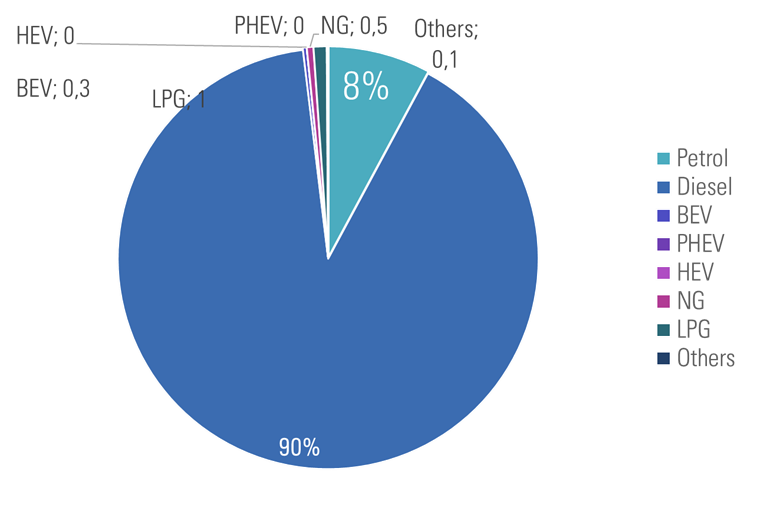
\includegraphics[width=0.8\textwidth]{Chapters/Pictures/grafico_diesel.png}
\caption{Powered Graph}
\label{fig:hdpower}
\end{figure}



So in compliance with the sustainability goals given by the UN it is necessary to renew also the Heavy duty compart. To do that we have 3 main options:
\begin{itemize}
    \item Biofuels
    \item Electric batteries
    \item $H_2$
\end{itemize}
As said the recent book \cite{Mazzo2021} the Electric batteries for Heay Duty are not so conviniebt so we will focus on the $H_2$ technologies.

-

\textit{In this section, provide a brief description of involved technologies, applications, state-of-the-art including actual size of systems, level of development, performances.}

\textit{Please, provide references/sources for the information in this section.}

\textit{3-6 pages (all the section)}

\section{Sate of the Art}